% Chapter 2 of the Thesis Template File
%   which includes bibliographic references.

%Chapter 2: Related Work  
%1) Introduction paragraph summarizing the flow/content/structure of the Related Work, while describing how the areas of related work are logically connect to your work  
%2) Related area 1 
%3) Related area 2  
%4) Related area 3
%5) Within each related area, point out in what why your work is different from the existing work.

\chapter{RELATED WORKS}\label{ch:relatedworks}

Three areas closely related to the work in this thesis are: digital radiometers, software defined radio based radiometers, and radio frequency interference (RFI) mitigation.  This chapter first presents two classifications of digital radiometers (hybrid and direct sampling).  Next, software defined radio based radiometers are discussed in their own section, as a third classification of digital radiometer.  This chapter concludes with a brief overview of the topic of RFI, which is important to consider when deploying radiometers.

\section{Digital Radiometers}

A digital radiometer replaces portions of a traditional radiometer's analog components with digital components[\cite{Ruf}].  Two types of digital radiometers include: hybrid and direct sampling.

\emph{Hybrid.}  A hybrid radiometer uses a mixture of  analog and digital components[\cite{skou}].  Often the analog voltage output from the diode of a square law detector, which is used to indicate the total power observed, will be digitized. 

\emph{Direct Sampling.}  A direct sampling radiometer can be considered a type of hybrid radiometer that directly samples the incoming RF signal and then uses digital signal processing techniques to extract total power information.  As an example, Iowa State University (ISU) owns a 1.4 GHz, dual polarization, correlating radiometer that uses direct sampling.  It was built by the University of Michigan and put into service at ISU in 2006 [\cite{Erbas}].  This radiometer takes the RF signal and using analog components amplifies and filters the signal, and then sends it to an analog to digital converter.  The radiometer is designed to operate in the protected spectrum of 1400 MHz to 1420 MHz.  Unlike other radiometers discussed, this radiometer samples the incoming RF signal at 1400 MHz.  This method allows for power information to be extracted, however the full signal can not be recreated due to Nyquist's theorem [\cite{Fischman2001}].

%When the  the ISU radiometer was built, an analog to digital converter (ADC) that could sample accurately at 1.4 GHz were expensive and not easily obtainable.  Since this radiometer was only interested in power information, it could under-sample at 1.4 GHz.  The samples are sent to a Field Programmable Gate Array (FPGA) to extract power information.  The correlation stage is another place where a radiometer could be digitized.  [\cite{Fischman2001}]. 

Both hybrid and direct sampling radiometers are designed to retain only the total power information contained in a RF signal.  While measuring total RF power is the primary purpose of a radiometer, as it will be discussed later, retaining phase and frequency information can be useful as well.

\section{Software Defined Radio Based Radiometers}

Software defined radio based radiometers can be considered a relatively new subclass of digital radiometer.  With the advent of software defined radios that are wildly available, there has been increasing interest in applying this technology to radiometers.  This section discusses two works that have explored using software defined radio technology in radiometry from the Shirley's Bay Radio Astronomy Consortium and from Grand Valley State University.

\emph{Shirleys Bay Radio Astronomy Consortium.}  The Shirleys Bay Radio Astronomy Consortium (SBRAC) made use of a software defined radio to restore a radio telescope used for radio astronomy.  They attached a software defined radio to their eighteen meter radius dish to obtain astronomical information by observing the hydrogen line located at 1420.4058 MHz in the RF spectrum[\cite{Leech2007}].  Marcus Leech, who headed SBRAC, contributed software to GNURadio specifically to support radio astronomy applications.  This branch of GNURadio was used as the software base used in this thesis [\cite{Leech}].

While parts of the GNURadio software used in this thesis were derived from Marcus Leech's work, additional features were added such as offending signal detection, offending signal detection, mitigation, and a software implemented noise generator.  Additionally, elements of the graphical user interface (GUI) were enhanced to aid in visualization and analysis data.  For example, a waterfall display of a signal spectrum over time was implemented.

\emph{Grand Valley State University.}  In 2013, the University of Illinois and Grand Valley State University built a software defined radio based radiometer to listen to emissions from Jupiter[\cite{Behnke}].  They custom built the hardware portion of their software defined radio using an Analog Devices analog to digital converter (AD9460) and a Xilinx (Spartan-3E-500) FPGA.  They also implemented a RF front end to filter and amplify the incoming RF signal.  The software side of their radiometer was composed of: 1) GNURadio for low-level communications with their software defined radio and, 2) Python script and WxGUI to implement a higher level user interface.  The students reported that their SDR based radiometer worked well at a low price point.  One aspect that differentiates the work in the thesis from Grand Valley State University's work is that they build their own custom hardware for their software defined radio, while in this work off the shelf components where used with an aim of making radiometers more wildly accessible to the research community.

\section{Radio Frequency Interference (RFI) Mitigation}
When an RF signal generated by a source other than the object (or phenomena) of interest interferes (i.e. masks or contaminates) with the RF signal of interest this is referred to as radio frequency interference (RFI).  Radio Frequency Interference (RFI) is a common problem with nearly all radiometers because they are highly sensitive receivers, thus even small unwanted signals can have a large negative impact on a radiometer based experiment.  It is for this reason certain frequency bands have been designated as protected frequencies' for radiometer use, by the international community.  However, not all entities abide by these standards.  For example, the satellite radiometer used by the Soil Moisture Ocean Salinity (SMOS) mission has had numerous issues with RFI [\cite{Kerr}] skewing their data and in some cases making the data unusable for soil moisture measurements [\cite{Richaume}].  

The area of RFI detection and mitigation is still an active field of research [\cite{Forte}].  With respect to RFI detection, since radiometers typically do not retain spectral frequency information, statiscal methods have been explored that loot at variations in the received power to determine when RFI is occurring.

One such method is the kurtosis statistic method[\cite{DeRoo}] (or polarization signature) method.  With respect to RFI mitigation, mechanical filters are used to selectively filter out the offending signals [\cite{DeRooRFI}].  

While mechanical filters are an effective means of RFI mitigation, they add both weight and complexity to the radiometer.  For example, multiple filters would be required to isolate and remove frequency bands that contain the offending signal(s).  One idea this thesis explores is making use of frequency information and software-based digital filters for RFI detection and mitigation.


%----------------------------------------------------------
% End of Chapter 2.  Anything below this is extra information

%For our software defined radiometer however, we are looking at the ground and we are using the radiometer for soil moisture instead of measuring stars and other points of interest in the sky.  While the fundamentals is the same for either radiometer some adjustments need to be made because a radiometer that is looking at the sky often sees a cooler brightness temperature whereas a radiometer looking at the ground sees a much warmer brightness temperature.  This is due to the albedo of the Earth having a much warmer noise temperature then what you find with radio astronomy[\cite{Tiuri}].

% The following is information pulled out some time ago.  If after the Re-org this is still not inserted, this will get deleted.

%The existing ISU radiometer RF Front end uses a series of cascading low noise amplifiers (LNAs) that increase the power from the antenna while contributing a minimum amount of noise to the system [\cite{Erbas}].  In addition, the current ISU RF front end uses bandpass filters to narrow the bandwidth to the desired 1400 to 1425 MHz that we wish to monitor.  While these are not needed with the addition of the software defined radio, since we can filter in software, they do not contribute much in terms of the noise temperature, and as passive components do not impact the performance of the radiometer as much as the LNAs do.

%{\begin{figure}[h!tb] 
%\centering
%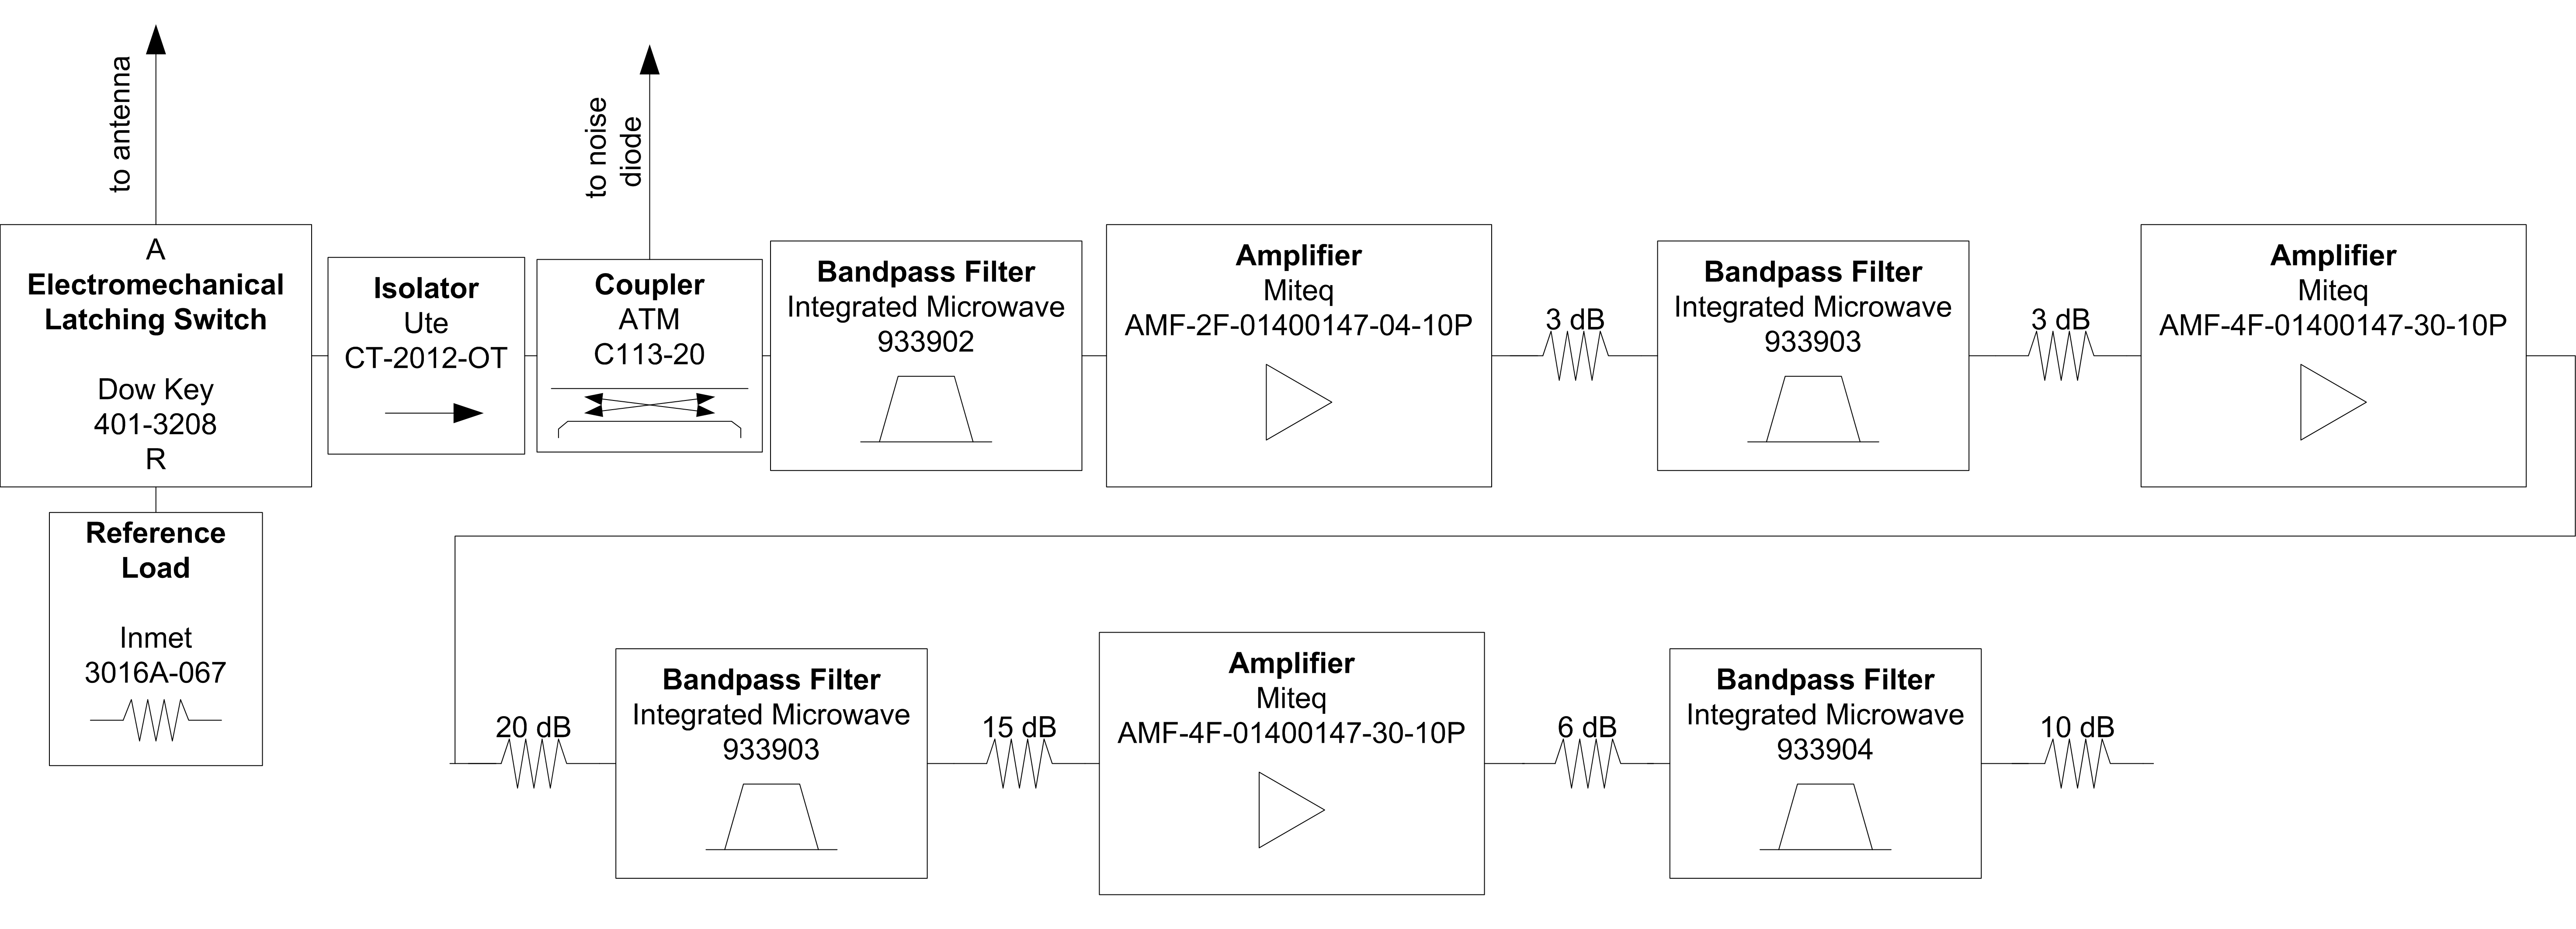
\includegraphics[width=17cm]{Images/ISU_rf_block.png}
%\isucaption{A block diagram provided by the University of Michigan that shows the components used in the ISU RF front end.}
%\label{ISU_rf_block}
%\end{figure}
%}

%As it can be seen in Figure \ref{ISU_rf_block} the current ISU rf front end uses a series of amplifiers, filters and attenuators to amplify and filter the incoming signals.  The attenuators are used to ensure that we do not overload the front end of the LNA proceeding it in the chain.  This RF chain provides us a spectrum from 1400 MHz to 1425 MHz and gives us a total gain of approximately 81 dBm.  This raises the noise floor to approximately -30 dBm which makes it very easy to detect with both a square-law detector and the software defined radio.  The performance of the ISU front end was confirmed by using a spectrum analyzer to look at the output signal and power output.  The spectrum analyzer output can be seen in Figure 

%{\begin{figure}[h!tb] 
%\centering
%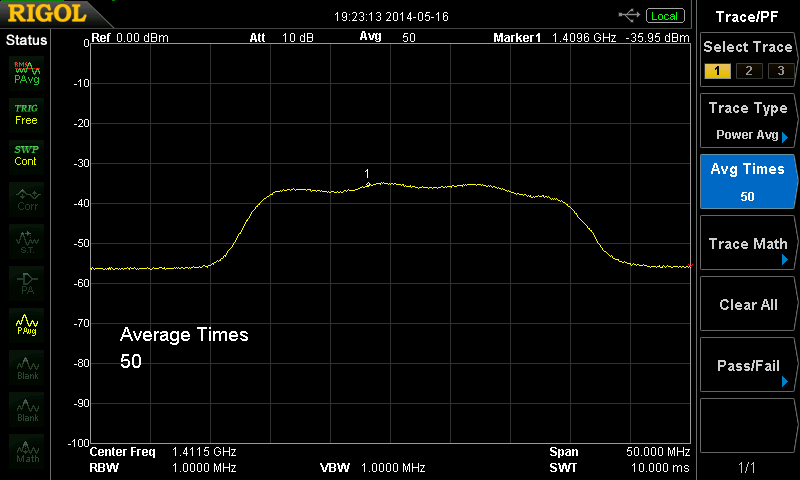
\includegraphics[width=17cm]{Images/radlidoff.png}
%\isucaption{A screenshot taken from a spectrum analyzer showing the filters and amplification done by the ISU Radio RF front end.}
%\label{ISU_rf_spectrum}
%\end{figure}
%}

%The ISU Radiometer front end was dismantled and was used for the experiments used in this thesis.  The LNAs and bandpass filters were kept intact to be used for experimentation.  While the bandpass filters were not needed for the software defined radio, since we were comparing our data to a square-law detector, they were still required for that device so that both the SDR and the Square-law detector could be looking at approximately the same signal.

